\subsection{Kommandozeilenprogramm Adobe-Illustrator-Designkonvertierung}

Wie bereits im Kapitel \ref{Der FreeDesign-Editor} \emph{Der FreeDesign-Editor} beschrieben, werden den Kunden Designvoralgen zur weiteren Gestaltung angeboten. 
Die Vorlagen von der Grafikabteilung mit dem Programm \emph{Adobe Illustrator} was eine Software zur Erstellung von Vektor-Grafiken ist \autocite[vgl.][]{Adobe:Illustrator}. Der Abschließende Schritt bei der Erstellung ist ein Export der Vorlagen im SVG-Dateiformat. Anschließend werden die SVG-Dateien durch einen Import-Prozess in das Easyprint-Shop-System importiert. Der FreeDesign-Design unterstützt diesen Prozess durch die Bereitstellung eines Kommandozeilenprogramms zur automatischen Konvertierung der SVG-Dateien, die durch \emph{Adobe Illustrator} erstellt wurden in Dateien, in Daten die durch FreeDesign-Editor gelesen werden können.  

Bereits im 

\begin{figure}[H]
    \centering
    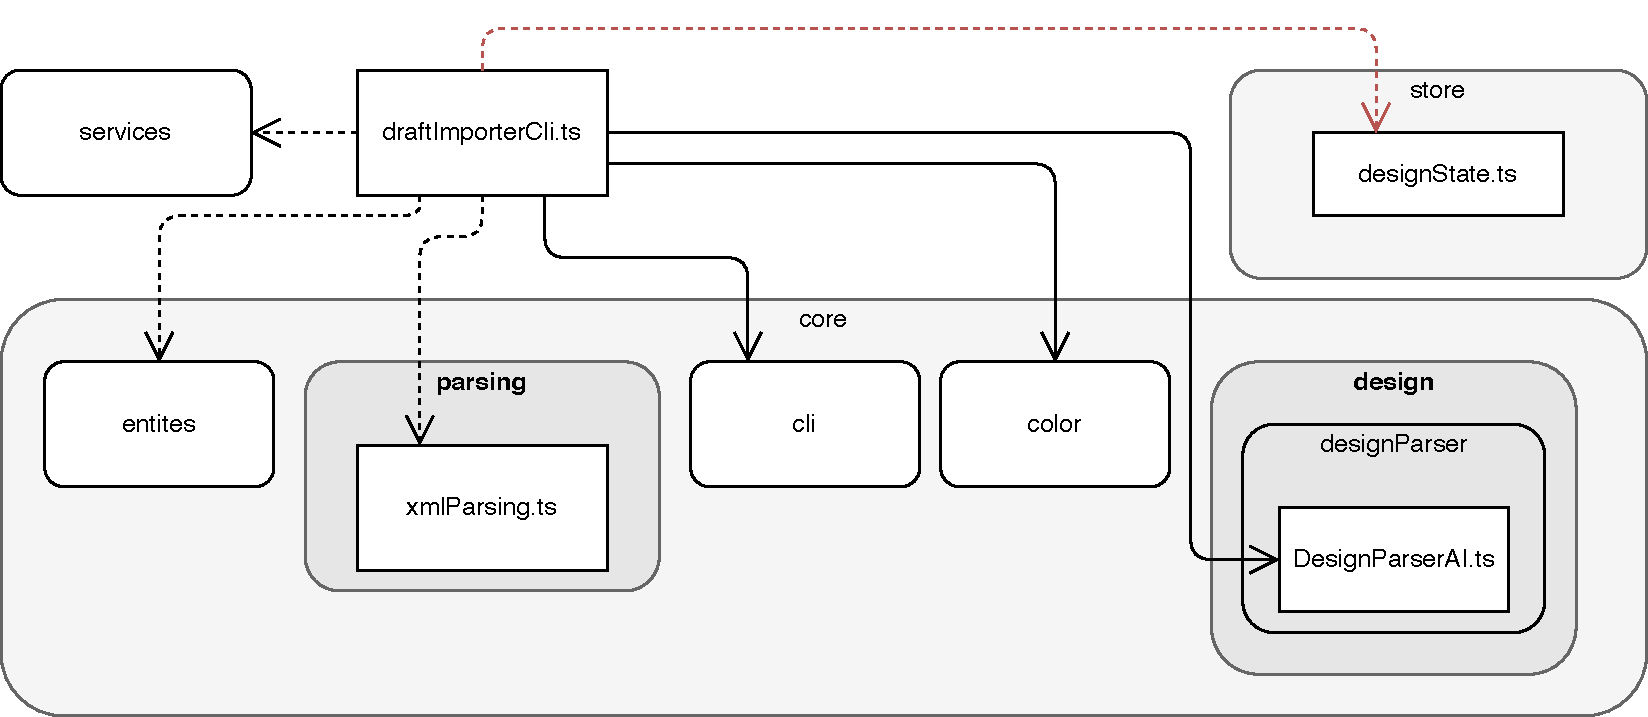
\includegraphics{diagrams/Ist-Architektur/draftImporter-analysis.pdf}
    \caption{Abhängigkeiten der Komponenten für das Kommandozeilenprogramm zur Konvertierung von Designs die mit Adobe-Illustrator erstellt wurden zu FreeDesign-Designs.}
    \label{fig:DesignImport}
\end{figure}

\begin{multicols}{2}    
    \begin{enumerate}
    \item API-Kommunikation
    \item Bildverarbeitung
    \item Cache
    \item Designstruktur
    \item Design-Parser
    \item Produktstruktur
    \item Farbstruktur
    \item JavaScript-Erweiterung
    \item Mathematik
    \item Maßeinheit-Konverter
    \item SVG-Parser
    \item Schriftverarbeitung
    \item XML-Parser
\end{enumerate}
\end{multicols}